 \chapter{GST材料的制备方法和特性研究}
\label{chap:03}

\section{采用磁控溅射制备GST薄膜}
\label{sec:exp}

本论文用磁控溅射的方法对纳米厚度的GST薄膜进行制备。本论文准备从溅射气压、溅射功率、溅射时间三个方面优化磁控溅射的条件。为了测量透射结构和反射结构并在这之间进行对比,每组相同的溅射条件下使用铝衬底和玻璃衬底各一进行溅射。其中,溅射气压可用0.2Pa, 0.3Pa, 0.5Pa, 0.6Pa四个参考值;溅射功率可用18W, 36W, 50W, 80W四个参考值;溅射时间可用5min, 10min, 15min, 20min四个参考值。如果采用完全实验,那么总共需要对$4 \times 4 \times 4 = 64$种不同条件下的样品进行溅射;而这其中可能只有若干片是接近符合要求的。为了节约工作量而又不失代表性,我们决定采用正交试验法 \cite{ortho} 来设计实验方案。根据正交试验法,我们需要做16次实验,这些实验的具体条件详见表 ~\ref{tab:ortho} 所示。
\begin{table}[htbp]
  \centering
  \caption{根据正交试验法 \cite{ortho} 确定的实验条件}
  \label{tab:ortho}
  \begin{minipage}[t]{0.8\textwidth} 
    \begin{tabular}{|c|c|c|c|}
    \hline
    序号 & 溅射气压/Pa & 溅射功率/W & 溅射时间/min\\
    \hline \hline
    1 & 0.2 & 18 & 5 \\
    \cline{1-4}
    2 & 0.3 & 18 & 10 \\
    \cline{1-4}
    3 & 0.5 & 18 & 15 \\ 
    \cline{1-4}
    4 & 0.6 & 18 & 20 \\ 
    \cline{1-4}
    5 & 0.2 & 36 & 10 \\ 
    \cline{1-4}
    6 & 0.3 & 36 & 15 \\ 
    \cline{1-4}
    7 & 0.5 & 36 & 20 \\ 
    \cline{1-4}
    8 & 0.6 & 36 & 5 \\
    \cline{1-4}
    9 & 0.2 & 50 & 15 \\
    \cline{1-4}
    10 & 0.3 & 50 & 20 \\
    \cline{1-4}
    11 & 0.5 & 50 & 5 \\
    \cline{1-4}
    12 & 0.6 & 50 & 10 \\
    \cline{1-4}
    13 & 0.2 & 80 & 20 \\
    \cline{1-4}
    14 & 0.3 & 80 & 5 \\
    \cline{1-4}
    15 & 0.5 & 80 & 10 \\
    \cline{1-4}
    16 & 0.6 & 80 & 15 \\
    \hline
    \end{tabular}
  \end{minipage}
\end{table}
根据正交试验法,如果将这三类参数看作三维空间,那么在64种条件下的实验可以看作这个三维空间的正方体以及其内部的各个格点;而正交试验法在这个正方体内对应的点是一些均匀分布的点,因此能够认为这16个点是全部64个点的一个比较有代表性的抽样。同时,对于每组条件溅射两个样片,一片在玻璃衬底上溅射,一片在铝衬底上溅射。溅射得到的部分样片见图 ~\ref{fig:sputtered} 。
\begin{figure}[H] % use float package if you want it here
  \centering
  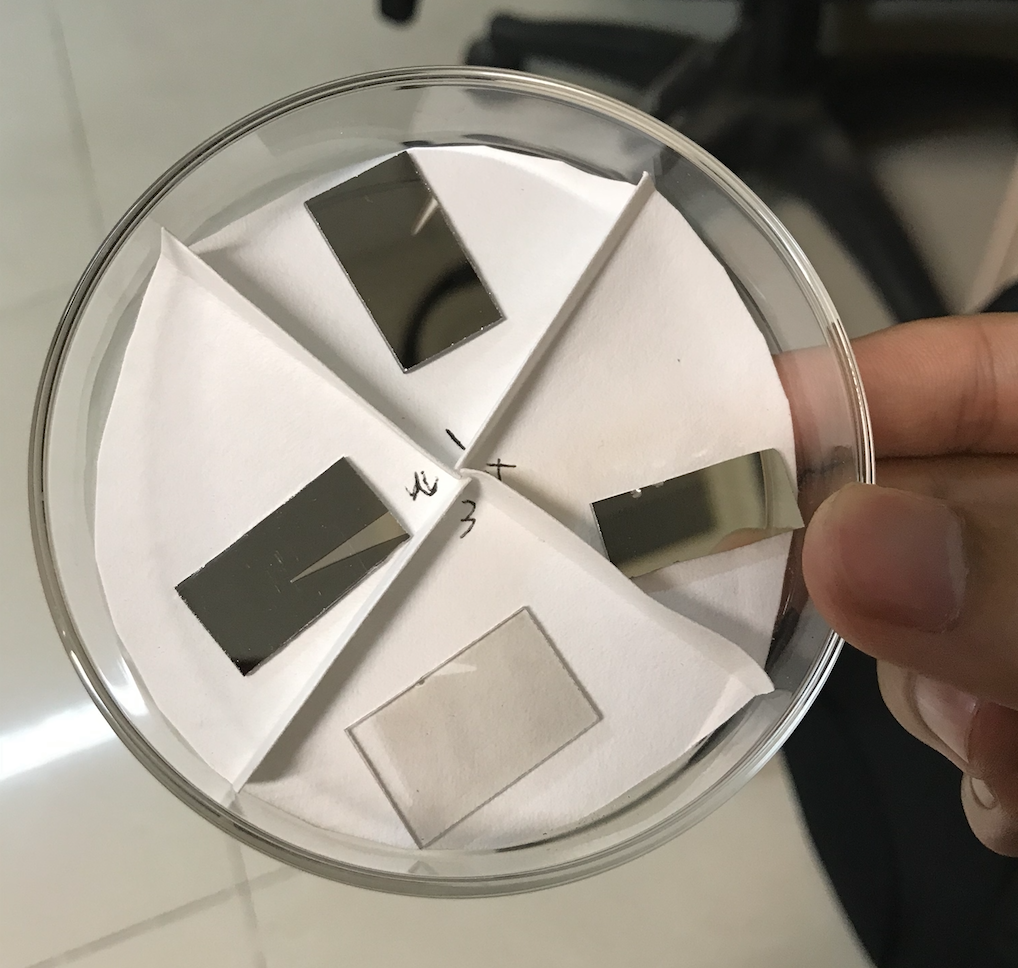
\includegraphics[width=0.5\textwidth]{sputtered.png}
  \caption{溅射得到的部分样片}
  \label{fig:sputtered}
\end{figure}
图 ~\ref{fig:sputtered} 中,一号是0.6 Pa, 36 W, 5 min的条件下在玻璃衬底上溅射的GST薄膜,二号是相同条件下在铝衬底上溅射的GST薄膜;三号是在0.3 Pa, 36 W, 15 min的条件下在玻璃衬底上溅射的GST薄膜,四号是相同条件下在铝衬底上溅射的GST薄膜。

根据得到的样片,我们可以看出在0.2Pa或者0.3Pa的氩气氛围中,溅射功率是18 W或者36 W的话,成膜速度相当慢,不适合用到实际工艺中。而在玻璃表面镀膜的话,当膜厚高于100nm时透明度就会下降到比较低的水准,因此GST材料不适合用作透射结构。根据傅立叶光谱仪的测试结果(详见 ~\ref{sub:testFourier})可以得到,溅射得到的GST薄膜中,材料处于非晶化状态。因此将样品直接做退火流程的时候首先要进行的是从非晶态向晶态转化的退火流程,即在300$\ ^{\circ}$C进行退火。

总体而言,用GST靶材在玻璃/铝衬底上进行磁控溅射均可以得到均一、平整的镀膜。其中经过台阶仪的测量结果,可以得到在0.5Pa, 80W的溅射条件下的成膜速率约为$35nm \cdot{} min^{-1}$并且在显微镜下观察得到的膜表面平整,此条件为本论文所采用。

\section{晶化条件研究}
\label{sec:RTA}
本论文选择热退火的方式来调节其晶化状态。又由于GST相变所需的温度不超过600$\ ^{\circ}$C,而这个温度下GST不易与氮气反应,所以无需采用真空条件下的管式炉进行退火,而采用氮气氛围下的快速退火。

我们得到了32片不同衬底上的GST材料。在每种溅射条件下选择一片进行退火,以便后续进行对比测试。经过300$\ ^{\circ}C$的RTA过程之后,进行了退火的16片样品中,有两片出现了不同程度的损伤。
\begin{figure}[H] % use float package if you want it here
  \centering
  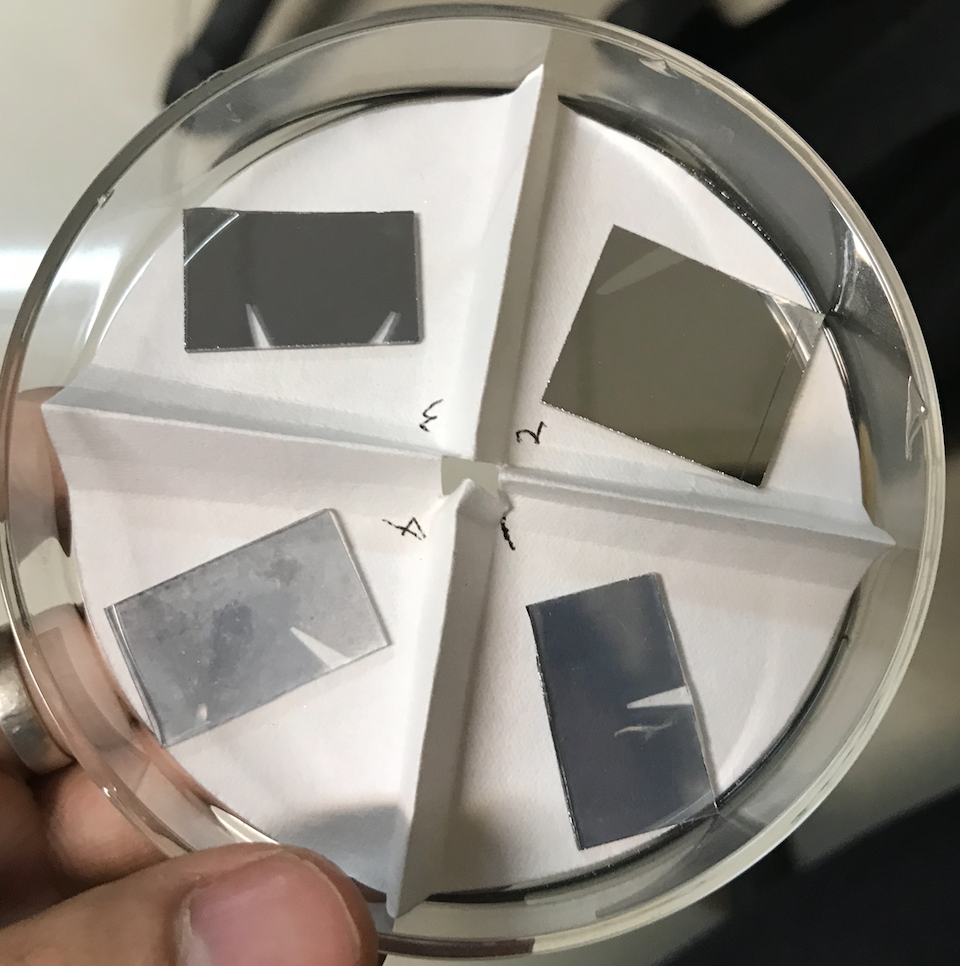
\includegraphics[width=0.5\textwidth]{RTAed.png}
  \caption{部分退火之后的样片形貌}
  \label{fig:RTA}
\end{figure}
由图 ~\ref{fig:RTA} 可以看出,编号为1和四的两片出现了不同程度的表面不平整的现象。由于出现问题的样片集中在直接将GST镀到玻璃上的,因此推断GST不适合直接在玻璃上进行溅射。因此在制备纳米厚度的GST薄膜过程中需要在玻璃上镀一层铝或者钛。

\section{厚度研究}
首先,我们关心的是溅射速度。为此,我们使用台阶仪来对厚度有一个直观的估计。台阶仪的原理之前已经提及过,在此不予赘述。在溅射功率为18W或者36W;同时溅射气压是0.2Pa或者0.3Pa时,即便在20min的溅射条件下也无法用台阶仪测得其准确结果,判断其厚度在100nm以下。实际上由于表面平整度和清洁程度的问题,能够看出明显台阶的只有若干片。其中较为典型的如下图所示:
\begin{figure}[H] % use float package if you want it here
  \centering
  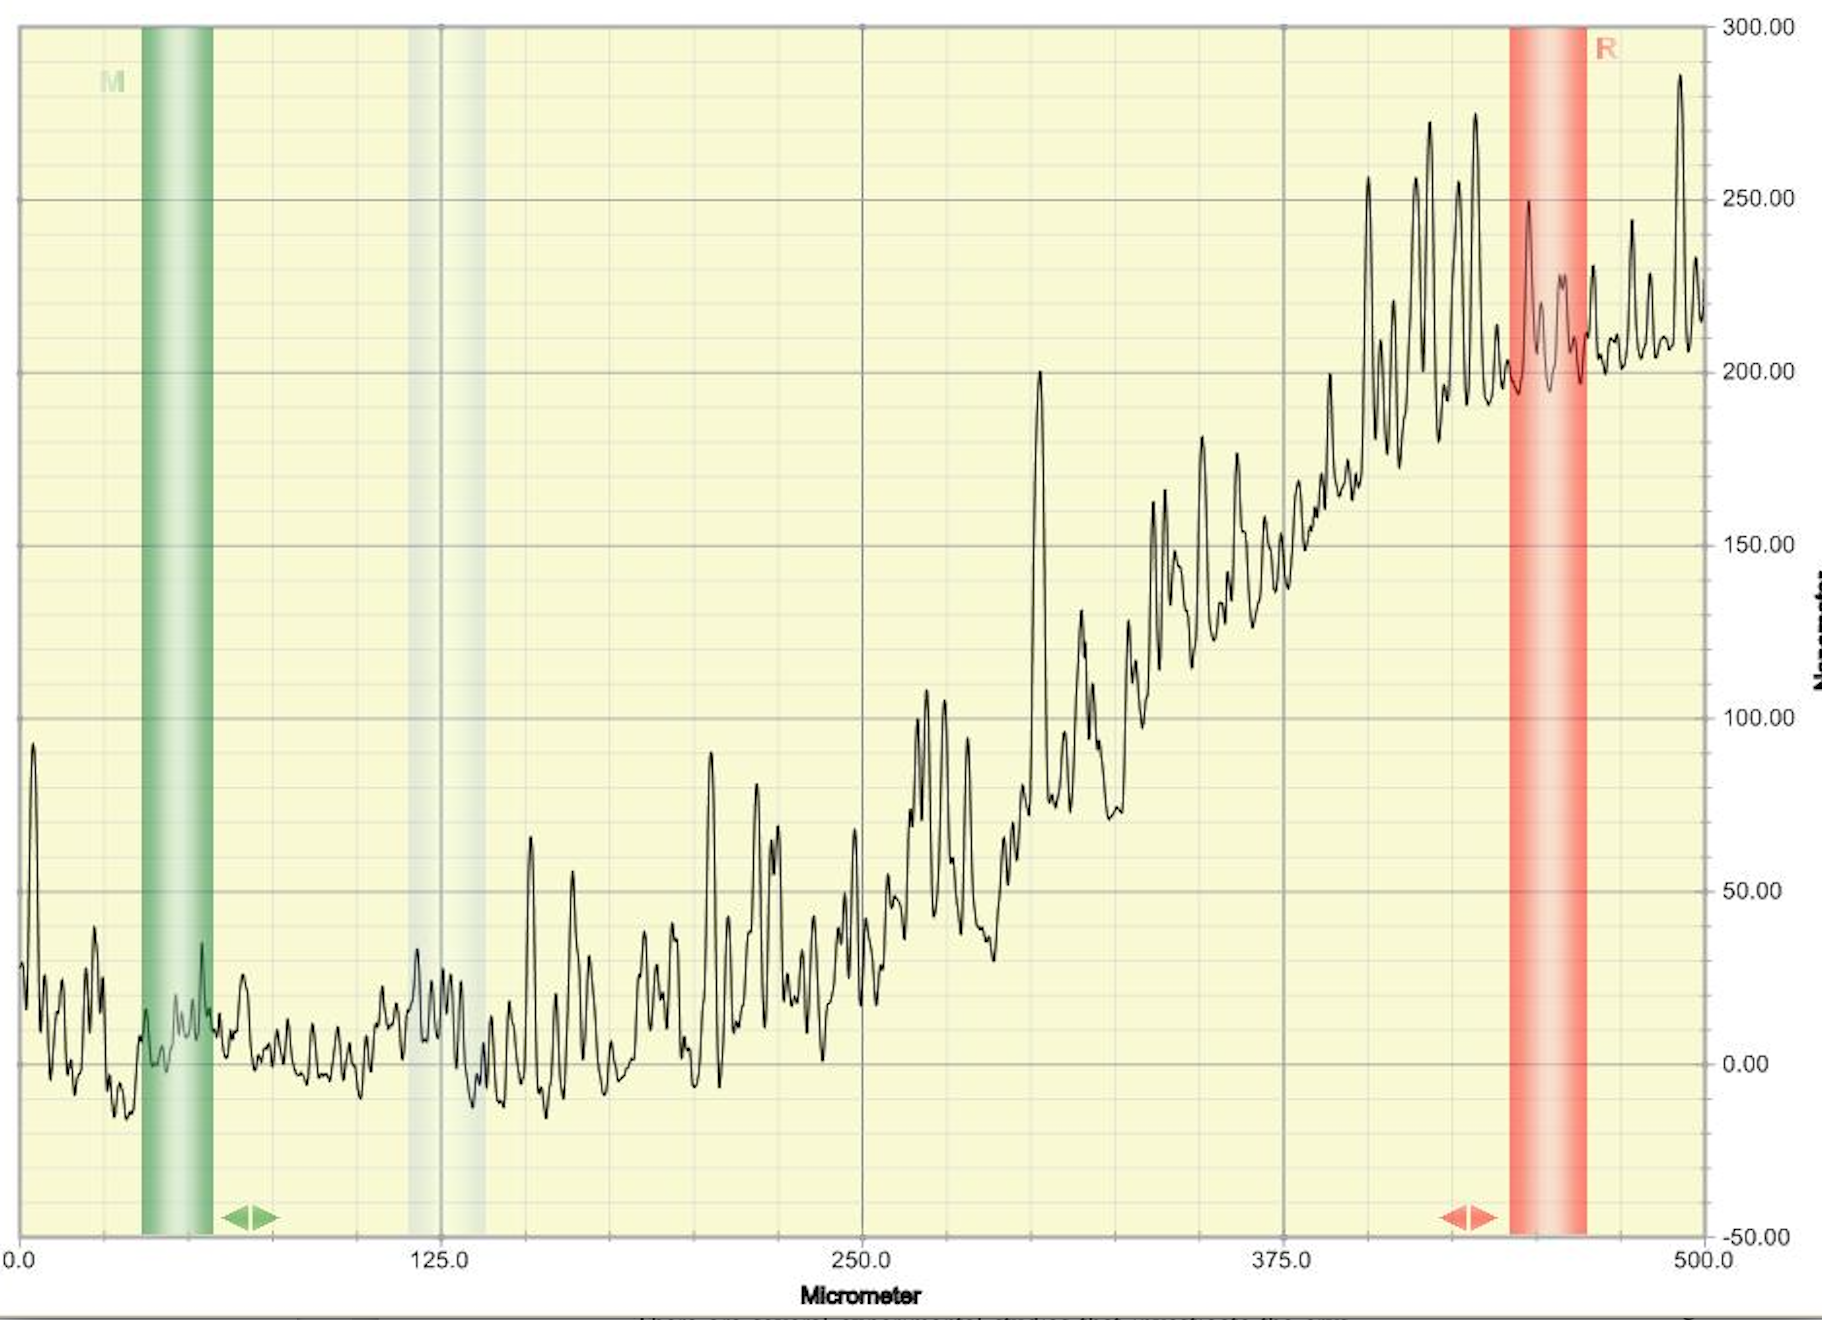
\includegraphics[width=0.5\textwidth]{GSTstep.png}
  \caption{溅射条件:50W,0.5Pa,5min}
  \label{fig:step}
\end{figure}
同时,当把溅射功率提升到80W的时候,溅射速率没有显著变化。由台阶仪的数据可以看出在这种溅射条件下,溅射速率约为$35nm \cdot{} min^{-1}$.

\section{光学特性测试}
\label{sub:testFourier}
本论文准备利用傅立叶光谱仪来测得GST材料的光学特性。其中,对于衬底是玻璃的GST膜,我们更关心它的透射特性;而对于衬底是铝的GST膜,我们更关心它的反射特性。经过测试,我们发现GST的透射特性基本随着波长的增加而增加,对于$\lambda \approx 1.4\ \mu m$以上的入射光基本可以视为透明材料(见图 ~\ref{fig:trans} )。

而对于铝衬底的GST膜,其反射率有明显的峰值,并且随着溅射条件(厚度)不同而不同,推测为光在上下表面发生干涉导致的(见图 ~\ref{fig:reflect})。
\begin{figure}[H] % use float package if you want it here
  \centering
  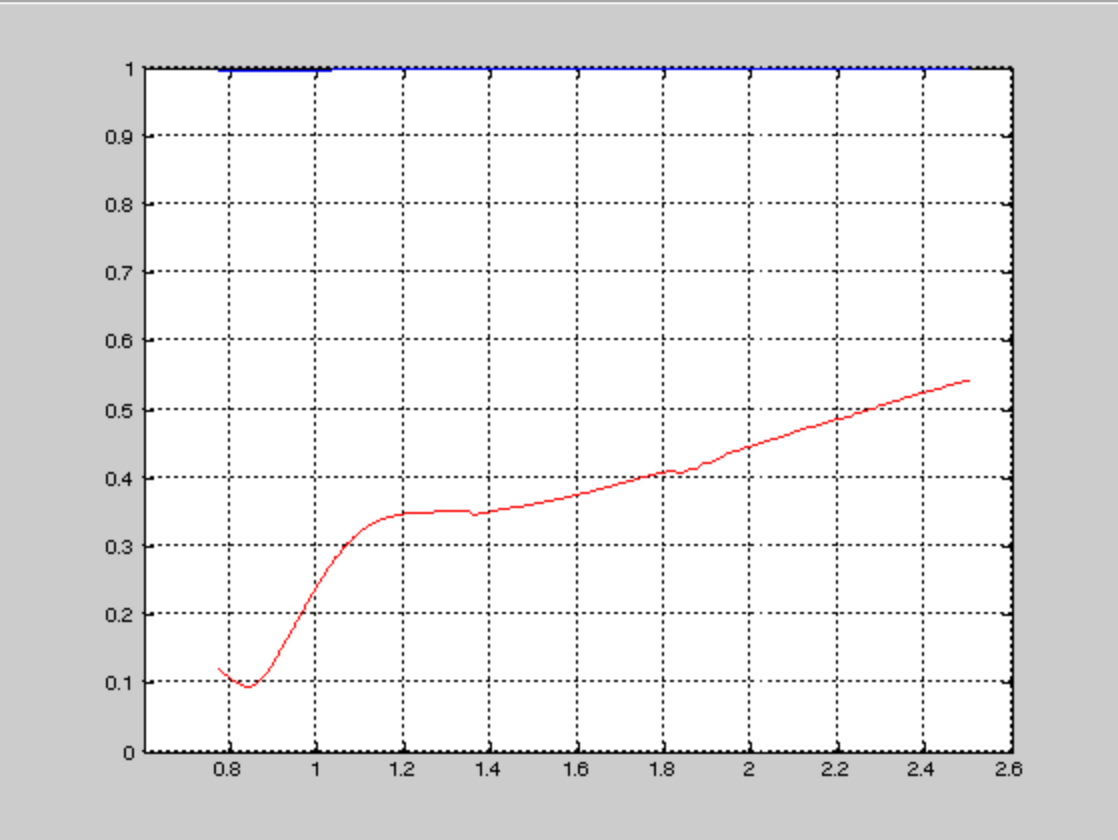
\includegraphics[width=0.8\textwidth]{GSTtrans.png}
  \caption{GST薄膜的透射曲线}
  \label{fig:trans}
\end{figure}
\begin{figure}[H] % use float package if you want it here??
  \centering
  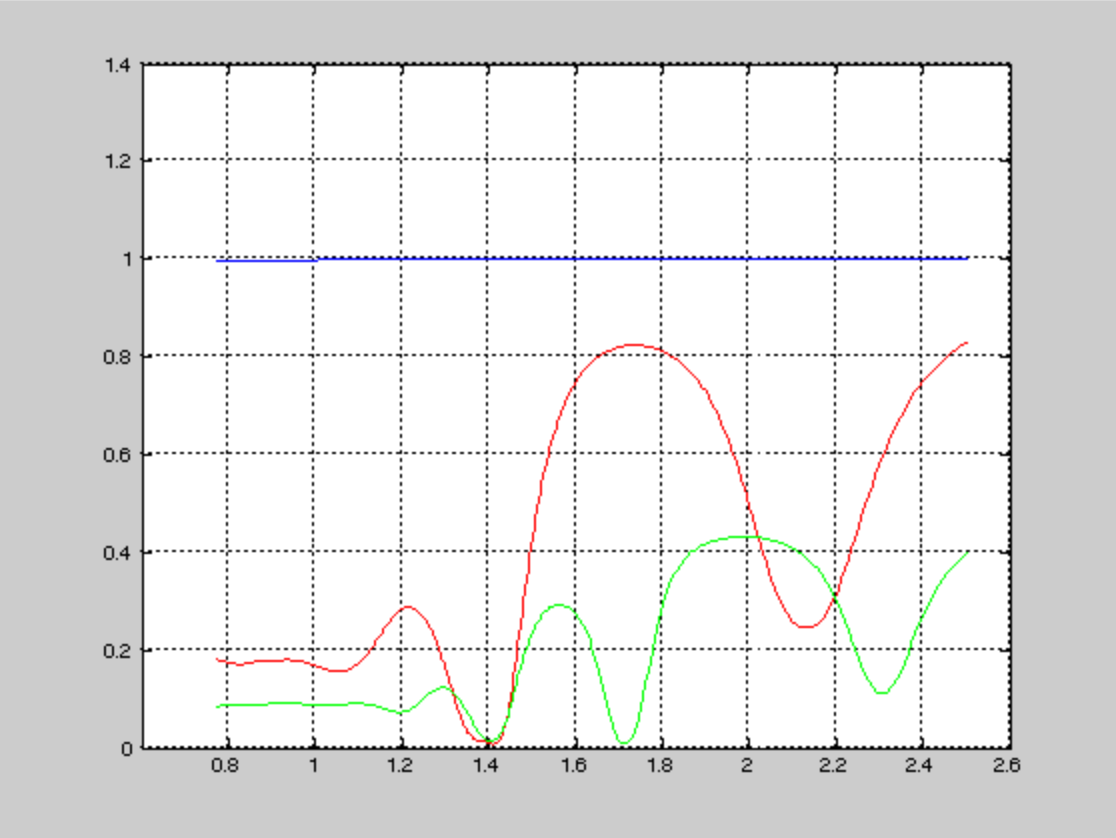
\includegraphics[width=0.8\textwidth]{GSTreflect.png}
  \caption{GST薄膜的反射曲线}
  \label{fig:reflect}
\end{figure}



\subsection{折射率测试}
本论文采用椭圆偏振仪测量GST薄膜的折射率,并以此推断材料的晶化状态,它和后面的XPS是我们判断退火是否有效的重要依据。
对椭偏仪的数据进行拟合的主要理论依据是柯西色散方程:
\begin{equation}
n\left ( \lambda \right ) = \sum_{i=0}^{\infty} \left (\frac{a_{k}}{\lambda ^{2k}} \right )
\end{equation}
在实际拟合过程中,我们只关心这个色散方程的前5项,以及薄膜厚度。拟合得到的曲线和椭偏仪测量的曲线总是存在较大的误差,可能的原因是各个部分的材料组分不稳定,或者材料表面不够平整。实际测得的GST材料的复折射率与最终拟合曲线和实测曲线的误差如下图所示:
\begin{figure}[H] % use float package if you want it here
  \centering
  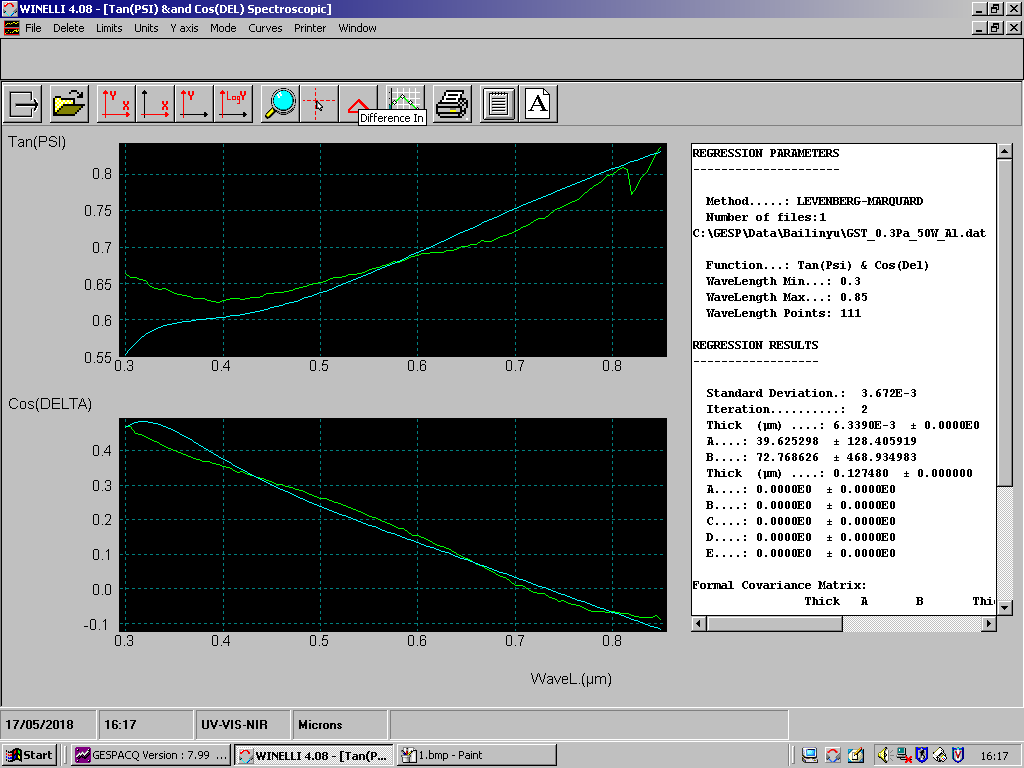
\includegraphics[width=0.8\textwidth]{ovaltest.png}
  \caption{拟合曲线和实测曲线的误差}
  \label{fig:oval}
\end{figure}
\begin{figure}[H] % use float package if you want it here
  \centering
  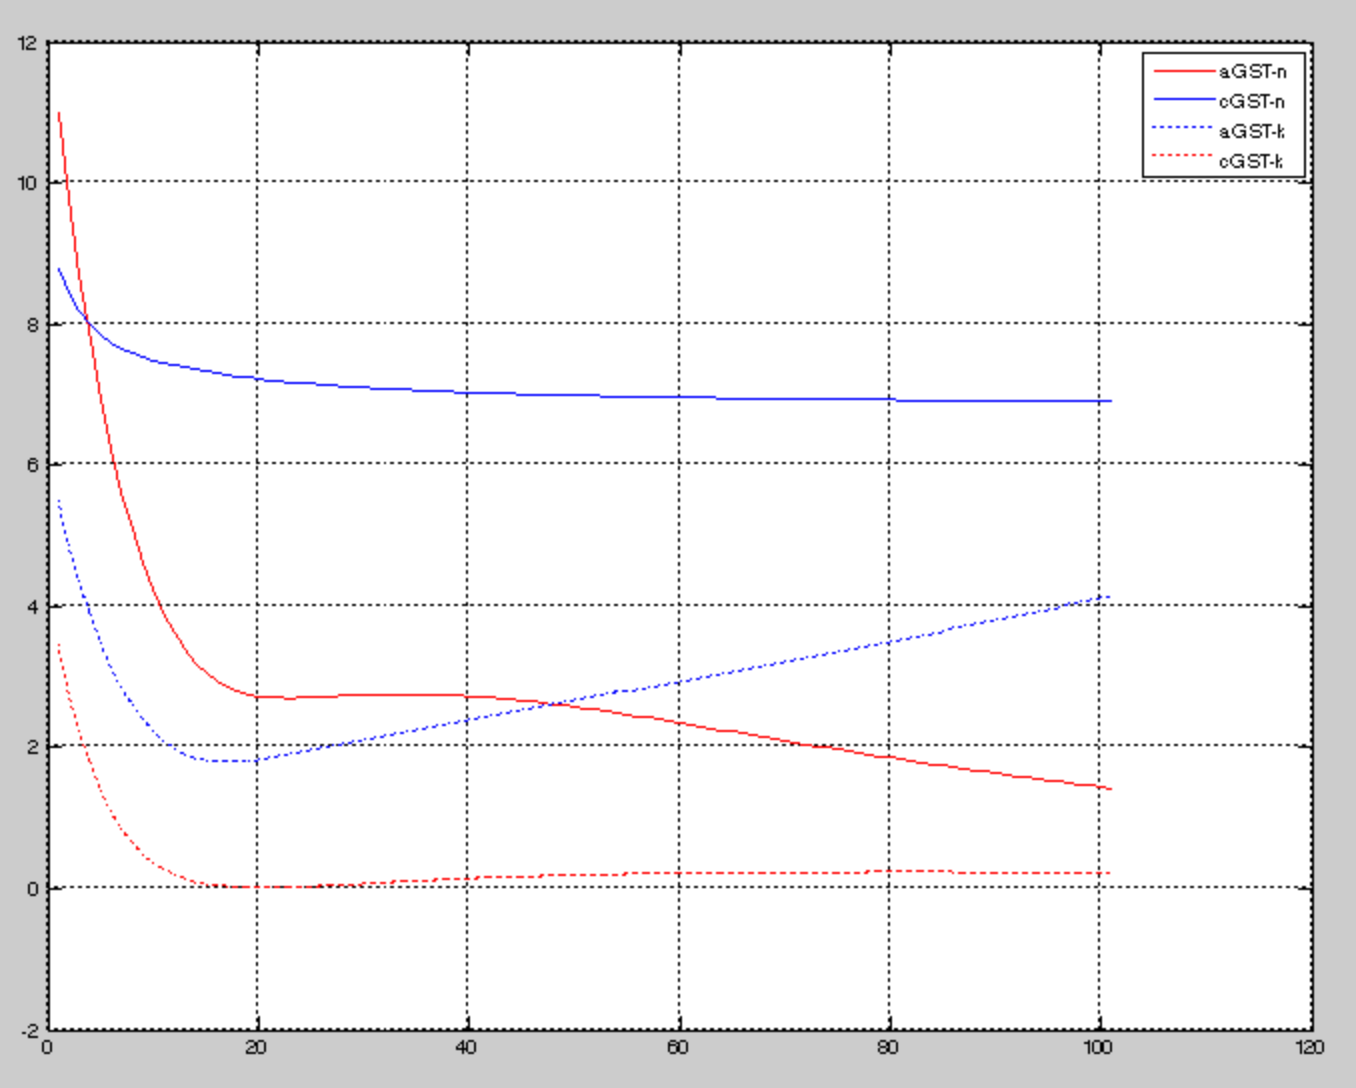
\includegraphics[width=0.8\textwidth]{GSTnktested.png}
  \caption{拟合结果对应的GST复折射率}
  \label{fig:nktested}
\end{figure}
\begin{figure}[H] % use float package if you want it here
  \centering
  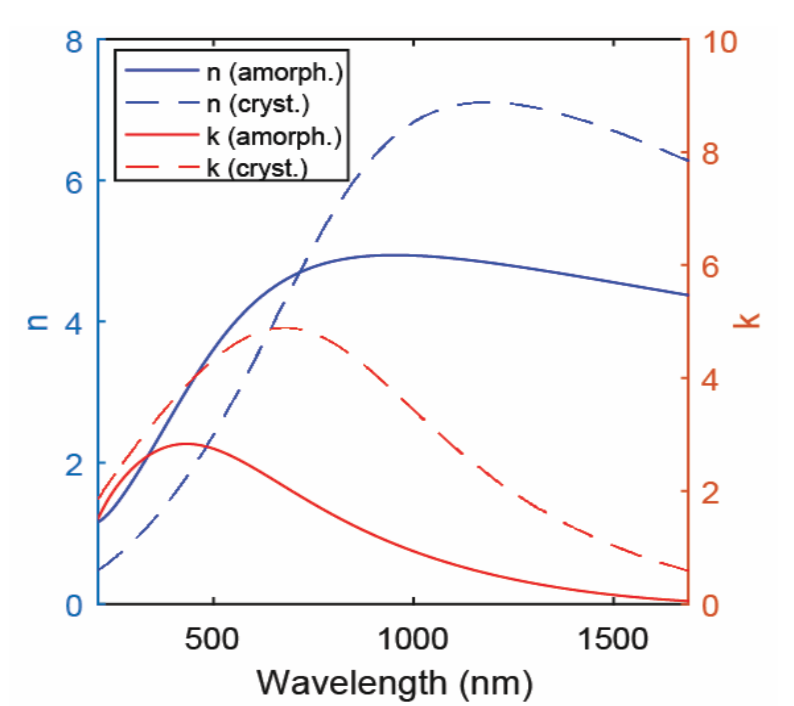
\includegraphics[width=0.5\textwidth]{GSTnk1.png} \cite{GSTnk}
  \caption{文献\cite{GSTnk}中给出的GST复折射率}
  \label{fig:nkGST}
\end{figure}


由以上数据并将上述数据和文献中的数据进行对比,我们可以发现尽管测得的GST复折射率同文献中提及的在数值上表现得较为接近,但是与预想的曲线存在趋势上的差距。在后续研究中,制作更为干净、更为平整的GST薄膜以及提升衬底金属的质量;同时,对柯西色散曲线的拟合可能需要尝试更多的初值,或者考虑尝试更多的色散模型来对椭偏仪测量得到的数据进行更准确的拟合。

\section{GST薄膜表面成分分析}
\label{sub:test_XPS}
本论文采用X射线光子能谱来对溅射得到的GST薄膜表面成分进行分析,以下是分析结果:
\begin{table}[htbp]
\centering
\caption{XPS测试结果}
\label{tab:subtable}
\subcaptionbox{GST未退火时的表面组分}
{
\begin{tabular}{|c|c|}
\toprule[1.5pt]
元素类型与轨道电子 & 含量百分比 \\
\midrule[1pt]
C1s & 28.04 \\
\hline
O1s & 49.02 \\
\hline
Ge2p & 4.75 \\
\hline
Sb3d & 3.61 \\
\hline
Te3d & 14.58 \\
\bottomrule[1.5pt]
\end{tabular}
}
\hskip1cm
\subcaptionbox{退火后的GST表面组分}
{
\begin{tabular}{|c|c|}
\toprule[1.5pt]
元素类型与轨道电子 & 含量百分比 \\
\midrule[1pt]
C1s & 24.8 \\
\hline
O1s & 58.48 \\
\hline
Ge2p & 3.74 \\
\hline
Sb3d & 4.28 \\
\hline
Te3d & 8.71 \\
\bottomrule[1.5pt]
\end{tabular}
}
\end{table}
\\
通过 ~\ref{tab:subtable} 的结果可以得到,无论GST薄膜是否经过退火,表面都有大量的碳、氧杂质。其中,碳的引入是必然的,因为XPS测试通常使用碳原子进行定标;而氧的引入可能是因为从溅射/退火到后来送样期间时间较长,表面氧化严重。同时组分中Ge, Sb, Te的比例大致保持着$2:2:5$的化学计量数之比,这说明GST的各个组分之间在溅射前后相对稳定。同时,表层的氧原子含量过高,这点也可能和椭偏仪的测试结果不尽如人意有关。